The OpenQuake scenario risk calculator allows the user to employ more than one ground motion prediction equation (GMPE) for computing the hazard curves used for the loss curve calculation. The loss exceedance curves, expected losses over the specified time period, and insured loss curves (if any), are calculated and output for each GMPE branch independently. No sampling is involved, and any branch weights assigned to the different GMPE branches are ignored. This case is designed to test the computation of the loss curve and average annual loss for an asset with two different GMPEs. The two ground motion prediction equations used are \citet{boore2008}, and \citet{chiou2008}.

A single asset is used in this test case. Table~\ref{tab:vf-ln-tax1-nzcov} shows the mean loss ratios and corresponding coefficients of variation in the vulnerability function used in this test case. The loss curve calculation procedure follows the same steps as described earlier in Case~1c for each of the two individual hazard branches.

The expected loss curves for this case, computed using the procedure described in Case~1c, are compared with the loss curves obtained using the OpenQuake classical PSHA based risk calculator in Figure~\ref{fig:lc-cr-7a}.

\begin{figure}[htbp]
\centering
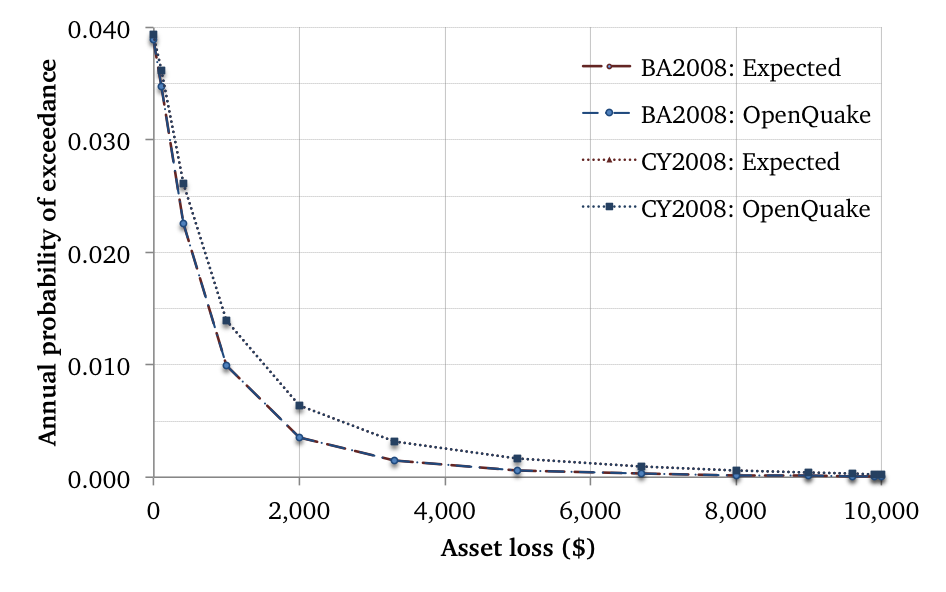
\includegraphics[width=12cm]{qareport/figures/fig-lc-cr-7a}
\caption{Loss curve comparison for classical risk test case 7a}
\label{fig:lc-cr-7a}
\end{figure}

The area under the loss exceedance curves gives the average annual loss values for the two hazard branches.